\chapter{Teknologi} \label{Teknologi}
I dette afsnit undersøges Ultralyds Robotarmen ud fra et teknologisk perspektiv.  \\
Den teknologiske løsning består af:
\begin{itemize}
\item UR3 Robotarm fra Universal Robots incl. software til styring af denne
\item Stativ til robotten
\item Joystick med dummy-probe
\item Computer
\item Holder til ultralydsprobe
\end{itemize}
Denne løsning skal kobles til det allerede eksisterende udstyr. Derfor er produktet en add-on løsning, hvilket betyder, at produktet skal købes udover det almindelige scanningsudstyr. Det eksisterende system består af Voluson S6 inkl. DICOM (Digital Imaging and Communications in Medicine) og en printer, samt diverse ultralydsprober, se Bilag 4 og Bilag 5.  

%Se bilag økonomi. 
\begin{figure}[H]
	\begin{minipage}{0.45\textwidth}
		\centering
		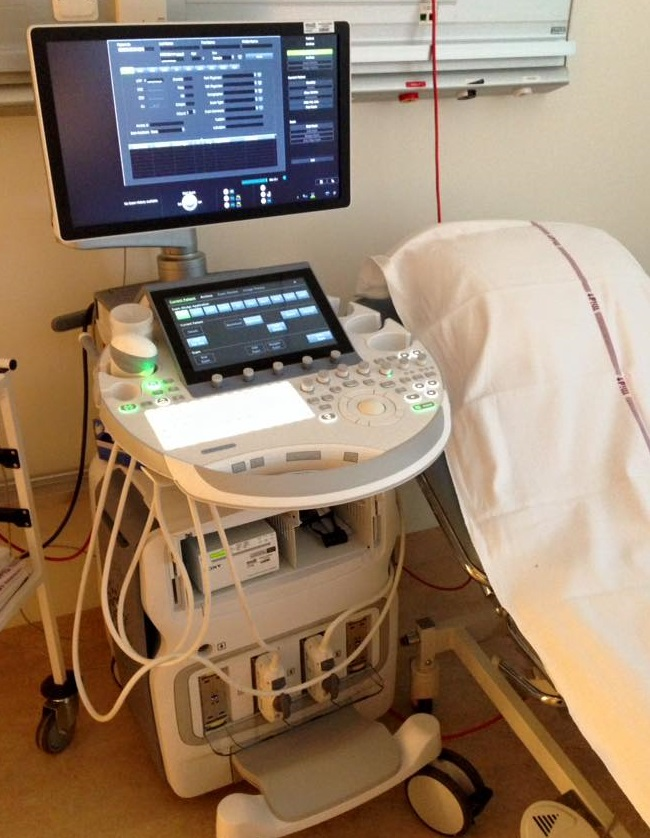
\includegraphics[width=\textwidth]{Figurer/udstyrHorsens.jpg}
		\caption{Nuværende udstyr: Voluson S6 med tilbehør. Billede fra HEH.}
		\label{udstyrHorsens}
	\end{minipage}
	\hspace{0.02\textwidth}
	\begin{minipage}{0.55\textwidth}
		\centering
		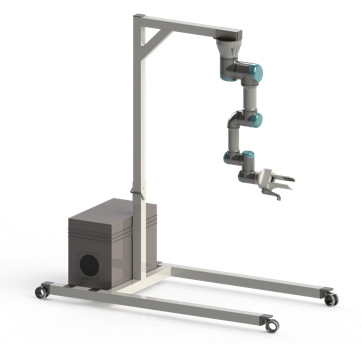
\includegraphics[width=\textwidth]{Figurer/StativMedUR3Render.png}
		\caption{Animation af robotarmen med stativ.}
		\label{Robotstativ}
	\end{minipage}
\end{figure}

\section{Anvendelsesområde}
Produktet skal anvendes til ultralydsscanninger af gravide patienter. Robotarmen er fastmonteret på et stativ, så den kan hænge over den gravide. Det medvirker til en større trykkraft, end hvis stativet stod på gulvet. For at skabe mobilitet, er stativet placeret på hjul. Hjulene kan låses af sikkerhedsmæssige årsager og for en statisk placering i forhold til den gravide. På robotarmen findes en universalholder til ultralydsproben. Holderen passer til alle større fabrikanters håndholdte ultralydsprober, bortset fra vaginalprober som robotarmen ikke kan bruges til, se Bilag 12, 28.04.2016.\\

Stativet med robotarmen skal være på den modsatte side af sengen end sonografen. Dette sikrer sonografens udsyn og kontakt til den gravide. \\
Robotarmen holder ultralydsproben over den gravide, mens den styres af sonografen via et joystick. Derved undgår sonografen fysisk akavede arbejdsstillinger.

Joysticket har en dummy-probe, som ikke har nogen probeegenskaber, som giver sonografen en følelse af at sidde med en ægte probe i hånden.
Systemet skal kunne overføre det tryk, som sonografen påvirker joysticket med, til robotarmen, se Bilag 12, 28.04.2016.
 

\begin{figure}[H]\centering
	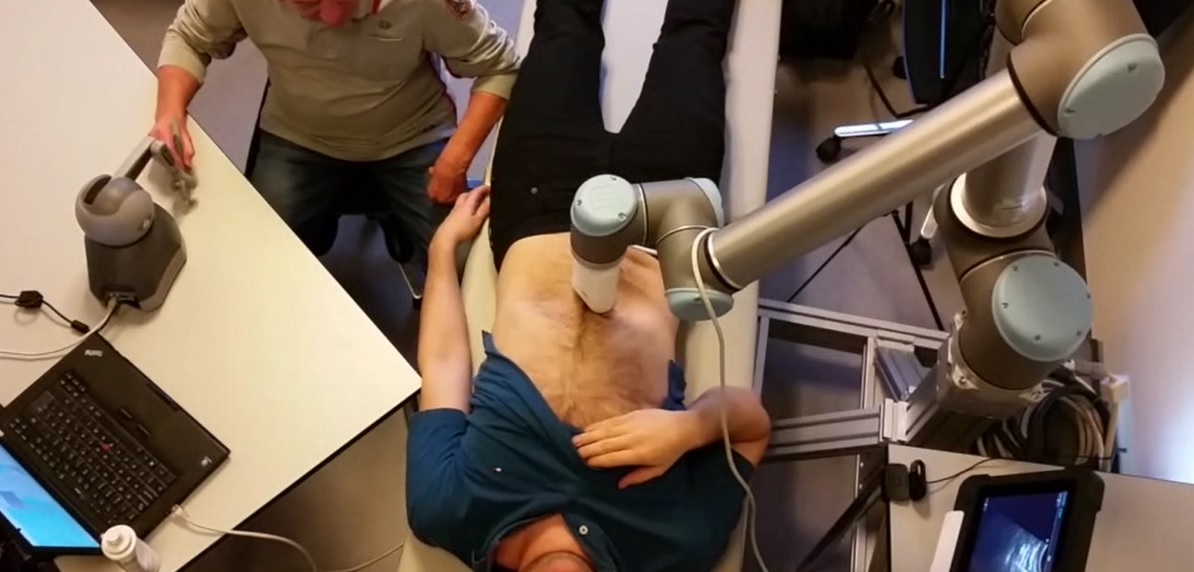
\includegraphics[width = 1.0\textwidth]{Figurer/ergonomiskLosning.jpg}
	\caption{Eksempel på opstilling af Ultralyds Robotarm. Nu er robotarmen placeret over patienten og ikke ved side af. På billedet ses joystick(tv.) og robotarm(th.).  }
	\label{ergonomiskLosning}
\end{figure}

\section{Specifikationer}
Robotarmen har en rækkevide på 50 cm, hvilket angiver hvor langt den kan række ud, som var det en arm. Den vejer 11 kg, derfor skal stativet være bygget dertil. Robotarmen har 6-graders frihed, som betyder at den kan bevæge sig i x-, y- og z-aksens retning og med drejevirkning om hver akse, se figur \ref{seksgradersfrihed}. Samtidigt kan den lave en +/- 360 graders rotation. \\
Robotarmen kræver en 100-240 VAC, 50-60 Hz strømforsyning, som betyder at den kan blive sat til en almindelig dansk stikkontakt, se Bilag 1.
  
\begin{figure}[H]\centering
	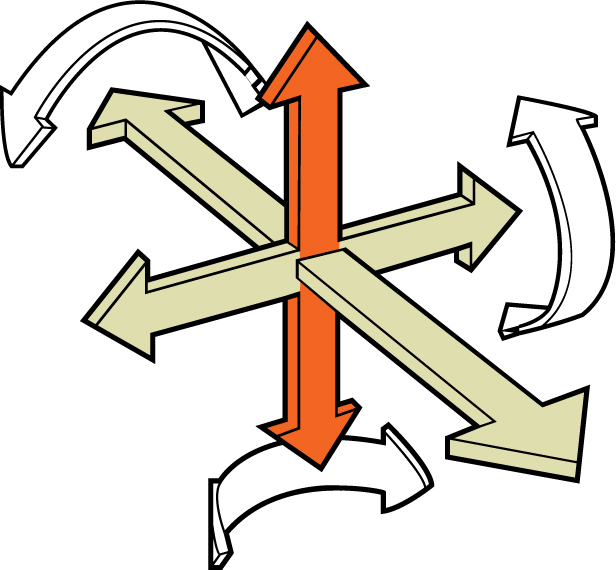
\includegraphics[width = 0.3\textwidth]{Figurer/sixDegressOfFreedom.jpg}
	\caption{Mulige retninger ved 6-graders frihed. Bevægelse i x-, y- og z-aksens retning og drejevirkning om hver akse \cite{6gradersfrihed}. }
	\label{seksgradersfrihed}
\end{figure}

Joysticket har bevægelighed som et håndled, derved har den også de begrænsninger som findes ved et håndled. Det har 6-graders frihed, se figur \ref{seksgradersfrihed}, så det passer med robotarmen, se Bilag 3. 

Der medfølger software til robotarmen, som er koblingslink mellem joystick og robotarm og styring deraf. Det er her bevægelserne fra joysticket omsættes til robotarmens bevægelser. Her er flere sikkerhedsmæssige foranstaltninger er placeret. Nogle er indbygget i robotarmen, for eksempel stopper den øjeblikkeligt, hvis den bliver mødt af en kraft på 50 N (ca. 5 kg) eller derover, se Bilag 2.    

\section{Effektivitet}
Det antages at Ultralyds Robotarmen vil blive benyttet til 70-80\% af scanningerne på gravide, da de sidste 20-30\% af scanningerne er for komplicerede til, at robotten kan udføre dem. Derfor skal sonografen manuelt foretage de sidste 20-30\% af scanningerne med den nuværende metode. \\ 
De komplicerede ultralydsscanninger er blandt andet scanninger på kvinder med højt BMI eller kvinder med bagoverbøjet livmoder, se Bilag 12, 28.04.2016. 
 
Ultralyds Robotarmen har ikke indflydelse på billedekvalitet eller kvaliteten af selve scanningen. Dette kommer af at ultralydsproberne er de samme, som man før har benyttet. \\
Computeren i Voluson S6 indeholder det samme software til billedanalyse og til diverse instrumenter som bruges under scanninger. Der er blandet andet tale om software til vækst- og flowmålinger af fostre.   \\
Når sonografen vil trykke med ultralydsproben på den gravide, vil trykkraften bliver overført til joysticket og dummy-proben så sonografen får den korrekte tryk feedback. Derved vil sonografen have følelsen af, at der bliver trykket direkte på patienten og kan dermed bedre selv have føling med situationen. \textbf{reference} 

\section{Sikkerhed}
I softwaren til styring af robotarmen findes en sikkerhedsindstilling, hvor en grænse for trykpåvirkningen skal indstilles. Hvis der af menneskelige eller tekniske fejl bliver påvirket med en kraft over grænsen, vil robotarmen automatisk slå fra og stoppe, se Bilag 12, 28.04.2016. \\
Som tidligere nævnt er der også en sikkerhed i, at robotarmen stopper sine bevægelser, hvis den bliver ramt af en kraft på over 50 N. Se Bilag 2. Denne foranstaltning gør, at den ikke vil gøre skade på mennesker eller genstande ved at ramme dem, samt at der ikke er behov for et eventuelt sikkerhedsgitter. 

\section{Delkonklusion}
Ultralyds Robotarmen kommer kun til at udføre 70-80\% af scanningerne, hvilket gør at sonograferne stadig skal udføre nogle af scanningerne manuelt. En stor del af belastningen på sonograferne fjernes, når robotarmen kan udfører størstedelen af scanningerne. Sonograferne vil have mere styrke til at udføre de mest komplicerede scanninger manuelt.

Der er tidligere blevet testet med robotarme i forbindelse med ultralydsscanninger, dog på hjertet. Her viste det sig ikke at være et problem at styre selve armen \cite{Hjerterobot}. Denne undersøgelse ligger nogle år tilbage i tiden, og derfor har teknologien allerede ændret sig meget. Det menes ikke at styring, betjening og implementering af Ultralyds Robotarmen til scanninger af gravide vil give de store problemer i sig selv som følge af ny teknologi. Der vil naturligvis altid være en overgangsperiode, hvor sonograferne skal vænne sig til at benytte teknologien. Under perioden vil en scanning muligvis tage længere tid at foretage, for at få den rette kvalitet på resultatet \cite{8}. 